\section{Monoidal objects in locally cubical bicategories}
\label{sec:mono-objects}

We now move on to define an appropriate abstract sort of ``monoidal object'' that will be preserved by the product-preserving functor $\cH$, and that specializes to monoidal double categories and to monoidal bicategories.
It would be nice if we could stay entirely in the world of iconic tricategories (that is, \Icon-enriched bicategories); but unfortunately the usual composition of monoidal functors between monoidal bicategories is not strictly associative, so they do not form an iconic tricategory.

However, they do form a more general structure, namely a bicategory enriched over \cDbl; in~\cite{gg:ldstr-tricat} this is called a \textbf{locally cubical bicategory}.
Since any bicategory can be regarded as a double category with only identity 1-morphisms, any iconic tricategory can be regarded as a locally cubical bicategory, but the latter are more general.
In particular, in a locally cubical bicategory the composition of 1-morphisms is associative only up to an invertible (vertical) 2-morphism.
And indeed, one of the results of~\cite{gg:ldstr-tricat} is that monoidal bicategories form a locally cubical bicategory; here we will generalize this to monoidal objects, perhaps braided and symmetric, in any iconic tricategory with finite products --- and indeed, in any locally cubical bicategory with finite products.

Since \cDbl\ is also a cartesian monoidal 2-category, we can define what it means for a locally cubical bicategory to have finite products, and this property is preserved when regarding an iconic tricategory as a locally cubical bicategory.
In particular, this applies to \cDblf\ and to \cBicat\ --- but actually, in place of the iconic tricategory \cBicat\ considered up until now we will focus instead on the locally cubical bicategory of bicategories constructed in~\cite{gg:ldstr-tricat}, whose ``locally horizontal part'' is \cBicat, but whose vertical 2-cells are \emph{icons}.
We denote this by \fBicat; it is easy to see that it also has products preserved by the inclusion $\cBicat\to \fBicat$, so that the composite functor $\cH : \cDblf \to\fBicat$ still preserves products.

We now define symmetric, braided and monoidal structures on objects, 1-cells, 2-cells, and 3-cells internal to a locally cubical bicategory with products, by taking the definitions of monoidal, braided, and symmetric structure for bicategories given in~\cite{nick:tricatsbook},~\cite{mccrudden:bal-coalgb}, and~\cite{gg:ldstr-tricat} and regarding the data of bicategories, functors, pseudonatural transformations, and modifications abstractly as objects, 1-cells, 2-cells, and 3-cells in a locally cubical bicategory.

Note that under this translation pseudonatural transformations become \emph{horizontal} 2-cells.
The horizontal 2-cells in \cDblf\ (which has no nonidentity vertical 2-morphisms) are the (vertical) transformations, while those in \fBicat\ are exactly the pseudonatural transformations (its vertical 2-morphisms are icons).
Let \fB\ be a locally cubical bicategory with products.

\begin{defn}
A {\bf monoidal object} in \fB\ is an object $A$, equipped with 1-cells $\otimes_A: A \times A \rightarrow A$ and $I_A: * \rightarrow A$, and 2-cells
\begin{itemize} 
\item $\alpha: \otimes \odot (\id \times \otimes) \Rightarrow \otimes \odot (\otimes \times \id)$
\item $l: \otimes \odot (I \times \id) \Rightarrow \id$ and $r:\otimes \odot (\id \times I) \Rightarrow \id$ 
\end{itemize}
Finally, it must be equipped with the invertible 3-cells $\pi, \mu, \lambda, \rho$, relating the two different ways around the Mac Lane pentagon and the three other coherence diagrams given in Definition 4.1 of~\cite{nick:tricatsbook}, which satisfy the appropriate three axioms.

A monoidal object is {\bf braided} if in addition there is a 2-cell $\sigma_A: \otimes \Rightarrow \otimes \circ \tau$, where $\tau: A \times A \rightarrow A \times A$ interchanges the two copies of $A$; and if there are invertible 3-cells 

\begin{equation}
  \begin{aligned}
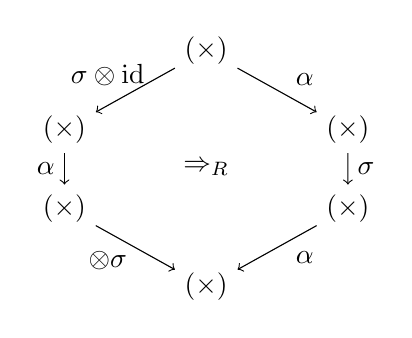
\begin{tikzpicture}[xscale=0.9]
\node (t) at (2,3) {$\ten (\ten \times \id)$};
\node (tl) at (0,2) {$\ten(\ten \times \id)$};
\node (bl) at (0,1) {$\ten (\id \times \ten)$};
\node (b) at (2,0) {$\ten (\id \times \ten)$};
\node (tr) at (4,2) {$\ten(\id \times \ten)$};
\node (br) at (4,1) {$\ten (\ten \times \id)$};
\draw[->] (t) to node [above,xshift=10pt, yshift=-2] {$\alpha$} (tr);
\draw[->] (tr) to node [right] {$\sigma$} (br);
\draw[->] (br) to node [below,xshift=10pt, yshift=2pt] {$\alpha$} (b);
\draw[->] (t) to node [above,xshift=-10pt, yshift=-2pt] {$\sigma \otimes \mbox{id}$} (tl);
\draw[->] (tl) to node [left] {$\alpha$} (bl);
\draw[->] (bl) to node [below,xshift=-10pt,yshift=2pt] {$\mathid \otimes \sigma$} (b);
\node at (2,1.5) {$\Rightarrow_{R \iso}$};
\end{tikzpicture}
  \end{aligned}
\hspace{5pt}\mbox{and} \hspace{5pt}
\begin{aligned}
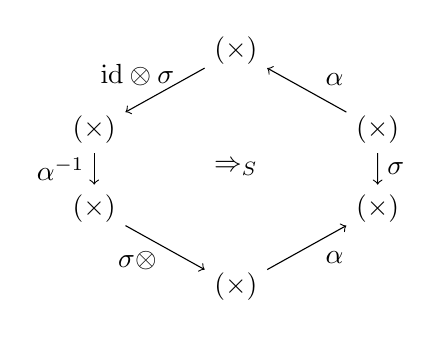
\begin{tikzpicture}[xscale=0.9]
\node (t) at (2,3) {$\ten(\id \times \ten)$};
\node (tl) at (0,2) {$\ten(\id \times \ten)$};
\node (bl) at (0,1) {$\ten(\ten \times \id)$};
\node (b) at (2,0) {$\ten(\ten \times \id)$};
\node (tr) at (4,2) {$\ten(\ten \times \id)$};
\node (br) at (4,1) {$\ten(\id \times \ten)$};
\draw[->] (tr) to node [above,xshift=10pt, yshift=-2] {$\alpha$} (t);
\draw[->] (tr) to node [right] {$\sigma$} (br);
\draw[->] (b) to node [below,xshift=10pt, yshift=2pt] {$\alpha$} (br);
\draw[->] (t) to node [above,xshift=-10pt, yshift=-2pt] {$\mbox{id} \otimes \sigma$} (tl);
\draw[->] (tl) to node [left] {${\alpha}^{-1}$} (bl);
\draw[->] (bl) to node [below,xshift=-10pt,yshift=2pt] {$\sigma \otimes \mathid$} (b);
\node at (2,1.5) {$\Rightarrow_{S \iso}$};
\end{tikzpicture}
\end{aligned}
\end{equation}
satisfying the axioms (BA1), (BA2), (BA3), and (BA4) given in~\cite[p136--139]{mccrudden:bal-coalgb} . 
It is {\bf sylleptic} when there exists an invertible 3-cell

 \[
 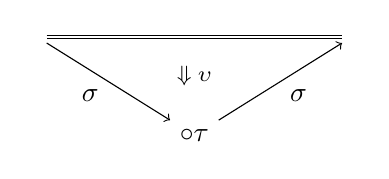
\begin{tikzpicture}
 \node (tl) at (-2,1) {$\ten$};
 \node (tr) at (2,1) {$\ten$};
 \node (b) at (0,-.25) {$\ten \circ \tau$};
 \draw[double] (tl)  -- (tr);
 \draw[->] (tl) to node[left, yshift=-5pt]{$\sigma$} (b);
 \draw[->] (b) to node[right, yshift=-5pt] {$\sigma$}(tr);
 \node at (0,0.5) {\footnotesize $\Downarrow \upsilon \iso$}; 
 \end{tikzpicture}
 \]
  satisfying the axioms (SA1), (SA2) on~\cite[p144--145]{mccrudden:bal-coalgb}. It is {\bf symmetric} if in addition, it satisfies the axiom given on~\cite[p91]{mccrudden:bal-coalgb}.
\end{defn}

By construction, these definitions give the expected results in \fBicat.
In \cDblf, where there are no nonidentity 3-cells, they reduce to the definitions from section~\ref{sec:symm-mono-double}; and in particular every syllepsis is a symmetry.

\begin{defn}
Let $A,B$ be monoidal objects in \fB. A 1-cell $f:A \rightarrow B$ is {\bf lax monoidal} when it is equipped with the following 2-cells:
\begin{itemize}
\item $\chi: \otimes_B \odot (f,f) \Rightarrow f \odot \otimes_A$
\item $\iota: I_B \Rightarrow f \odot I_A$
\end{itemize}
As well as invertible 3-cells $\omega, \gamma$, and $\delta$ given in Definition 4.10 of~\cite{nick:tricatsbook}, expressing the usual associativity and unitality conditions, which satisfy the two given commutativity axioms.
A monoidal 1-cell is called {\bf braided}, when $A$ and $B$ are braided and there is a 2-cell $u: \sigma_B \odot \chi  \Rightarrow \chi \odot f\sigma_A$, satisfying the braiding axioms analogous to (BHA1) and (BHA2) given in  \cite[p141-142]{mccrudden:bal-coalgb}. It is {\bf symmetric} when $A$ and $B$ are symmetric and the 3-cells defining the braided monoidal structure of $f$ satisfy the additional axiom analogous to  (SHA1) given in   \cite[p145]{mccrudden:bal-coalgb}.

When the natural transformations are in the opposite direction, the functor is {\bf oplax monoidal}, and when they are isomorphisms, the functor is {\bf strong monoidal}.
\end{defn}



\begin{defn}\label{Def:monverttrans}
Let $f, g:A \rightarrow B$ be monoidal 1-cells in \fB. A {\bf monoidal 2-cell} $\alpha: f \Rightarrow g$ is a (horizontal) 2-cell in \fB\ that is equipped with 3-cells
\begin{itemize}
\item $\Pi: \chi_f \odot \alpha \Rightarrow (\alpha \otimes \alpha) \odot \chi_g$
\item $M: \iota_f \odot \alpha \Rightarrow \iota_g$
\end{itemize}
such that the three coherence axioms in definition 3 of~\cite{gg:ldstr-tricat} hold.
A monoidal 2-cell is {\bf braided} or {\bf symmetric} when $f,g$ are braided or symmetric, and in addition the additional coherence axiom analogous to (BTA1) of~\cite[p143]{mccrudden:bal-coalgb} holds. Note that here the author writes $\rho$ for our braiding 1-cell $\sigma$.
\end{defn}

As remarked above, we will actually construct a locally cubical bicategory of monoidal objects.
The monoidal 2-cells will be the horizontal 2-cells therein; we now define the vertical 2-morphisms.

\begin{defn}
  Let $f, g:A \rightarrow B$ be monoidal 1-cells in \fB.
  A \textbf{monoidal icon} $\alpha: f \Rightarrow g$ is a (vertical) 2-morphism in \fB\ such that \dots [TODO].
\end{defn}

\begin{defn}
  A \textbf{monoidal 3-cell} is \dots [TODO].
\end{defn}

\begin{thm}
  Monoidal objects, lax monoidal 1-cells, monoidal 2-cells, monoidal icons, and monoidal 3-cells in \fB\ form a locally cubical bicategory, and similarly for colax and strong monoidal 1-cells and for braided, sylleptic, and symmetric objects and morphisms.
\end{thm}
\begin{proof}
  TODO.
\end{proof}


% Local Variables:
% TeX-master: "smbicat"
% End:
